\chapter{Interaction Region Local Coupling Correction in the LHC} % Main chapter title
\label{chapter:IR_Local_Coupling} % For referencing the chapter elsewhere, use \cref{chapter:IR_Local_Coupling}

% Previous chapters have covered how beam-based corrections of linear optics and nonlinear dynamics in colliders are essential for both beam control and in order to achieve the desired luminosity goals.
The linear optics and coupling correction usually constitute the first phase of machine commissioning as both are major contributors to the performance of colliders, and are required to be under good control for the next phases of commissioning.
In recent years, significant efforts have been made to improve the measurement and correction of linear and nonlinear global coupling both in the LHC~\cite{PRAB:Tomas:Review_Linear_Optics_Measurements, IPAC:Tomas:Measurement_Coupling_RDTs_LHC_AC_Dipole, PRAB:Calaga:Coupling_Merging_Hamiltonian_Matrix_Approaches, PRAB:Maclean:First_Nonlinear_Errors, PRAB:Maclean:Optics_Commissioning_Nonlinear_Era, PRAB:Persson:Chromatic_Coupling_Correction, PRAB:Tomas:ADECTA, IPAC:Maclean:ADECTA_Octupoles, PRAB:Biancacci:AC_Dipoles_Localize_Sources_Beam_Coupling_Impedance, CERN:Maclean:Demonstration_Coupling_Correction_Below_PerMil_LHC} and other synchrotrons~\cite{PRAB:Tian:Genetic_Algorithms_Storage_Ring, PRAB:Ohnishi:Measurement_Chromatic_XY_Coupling, PRAB:Carla:Local_Transverse_Coupling_Impedance_Measurements_Synchrotron_Light_Source, PRAB:Shen:Application_Independent_Component_Analysis_AC_Dipole_Based_Optics_Measurement_Correction_Relativistic_Heavy_Ion_Collider, PRAB:Sagan:Betatron_Phase_Coupling_Measurements_Cornell_Electron_Positron_Storage_Ring, PRAB:Fischer:Robust_Linear_Coupling_Correction_NTurn_Maps, ARXIV:Franchi:Error_Analysis_Linear_Optics_Measurements_Turn_Turn_Beam_Position_Data_Circular_Accelerators, PRAB:Tomas:Measurement_Local_Global_Resonance_Terms, NIMP:Yang:Method_Simultaneous_Linear_Optics_Coupling_Correction_Storage_Rings_Turn_Turn_Beam_Position_Monitor_Data, NIMP:Xiaobiao:Online_Optimization_Accelerators, IEEE:Raka:Measurement_Linear_Coupling_Brookhaven_AGS, PRAB:Franchi:Vertical_Emittance_Reduction_Preservation_Electron_Storage_Rings_Resonance_Driving_Terms_Correction, NIMP:Aiba:Ultra_Low_Vertical_Emittance_SLS_Systematic_Random_Optimization}, as its effect can lead to instabilities and unwanted dynamics in the machine~\cite{IPAC:Maclean:Effect_Coupling_Nonlinear_Observables, PRAB:Carver:Transverse_Instabilities_With_Coupling, PRAB:Franchi:Emittance_Sharing_Coupling, EPAC:Metral:Destabilising_Effect_Linear_Coupling_HERA_Proton_Ring, PRAB:Biancacci:AC_Dipoles_Localize_Sources_Beam_Coupling_Impedance}.

In the LHC local coupling correction has so far been done with the SbS technique~\cite{PRAB:Tomas:CERN_LHC_OMC}.
The method, however, suffers inherent weaknesses making it not local enough for coupling corrections.
This chapter, which constitutes the core of this thesis, presents a new method that was developed to determine corrections of linear coupling at the IPs.
An overview of the various experimental measurements taken for this work can be found in \cref{appendix:measurement_fills}.

%----------------------------------------------------------------------------------------

\section{Local Betatron Coupling in the LHC Interaction Regions}
\label{section:local_ir_coupling}

In the LHC, corrections of local IR linear coupling are of importance to keep a good control of beam sizes at the IPs and hence the luminosity performance, as well as to prevent a significant impact on the beam dynamics.

In \cref{equation:coupling_rdts_from_skew_quads} the contribution of elements to the linear coupling RDTs is given, where contributing elements are typically skew quadrupoles and solenoids.
The amplitude of the contribution is dominated by the integrated strength of the magnet \(k L\) as well as the \(\sqrt{\beta_x \beta_y}\) term at the location of the magnet.
Given that a tilted quadrupole interacts with the beam as a straight quadrupole with an additional skew quadrupolar component, once can see from \cref{figure:ir5_and_around} that any tilt in the triplet quadrupoles would generate a massive contribution to the coupling RDTs due to the very high \(\beta\)-functions in these magnets.

\Cref{figure:triplet_tilts_to_rdts} shows the coupling RDTs' amplitudes from tilts in triplet quadrupoles, with the \(\beta^{\ast} =\)~\qty{30}{\centi\meter} \num{2022} optics~\cite{CODE:acc-models-lhc}.
In this MAD-X simulation triplets around IP\num{1} were assigned random tilts within \(\pm\)~\qty{1.5}{\milli\radian}, and these were the only contribution to coupling in the machine.
Nevertheless, this contribution amounted to a \(\abs{C^{-}}\) of \num{3.84e-2}, too high for machine operation.

\begin{figure}[!htb]
    \centering
    \includegraphics*[width=0.99\textwidth]{Figures/IR_Coupling_Correction/triplet_tilts_to_rdts.pdf}
    \caption{Amplitudes of the coupling RDTs (bottom) \(f_{1001}\) (\textcolor{mplblue}{blue}) and \(f_{1010}\) (\textcolor{mplorange}{orange}) from tilts in the triplet quadrupoles around IP\num{1}. The top plot shows the magnets' powering while the middle plot shows the assigned tilts in each element.}
    \label{figure:triplet_tilts_to_rdts}
\end{figure}

As a consequence, the IR contribution - mainly the triplets - to global coupling needs to be compensated.
For this, in the LHC the local coupling correction is done by measuring the RDTs in the vicinity of the IP and using the MQSX skew quadrupole correctors introduced in \cref{subsection:lhc_eirs} and showcased in \cref{figure:ir5_and_around,figure:lhc_ir_corrector_layout} for correction.
The corrections are determined with the Segment-by-Segment technique described in \cref{subsection:correction_principles}, and try to cancel the triplets' contribution as well as possible.
Though this compensation is rarely perfect, the residual contribution is usually small enough to be handled by the skew quadrupole correctors present in the LHC arcs (see \cref{subsection:lhc_arcs}).
This correction is essential in order to reach low \(\beta^{\ast}\) with good optics control: at \(\beta^{*}=\) \qty{30}{\centi\meter} the local errors compensated in Run~\num{2}~\cite{CERN:Persson:LHCOpticsCorrectionsEvian2019} would contribute to the \(\abs{C^{-}}\) by the amount of \num{0.33}, too high for the arc correctors to handle.
While such coupling in the machine is not inherently unstable in itself, it leads to other effects causing the machine to be unstable such as transverse instabilities from loss of Landau damping~\cite{MASTERS:Soubelet:Optics_Octupole_PyHEADTAIL,PRAB:Carver:Transverse_Instabilities_With_Coupling}.

Due to their location the MQSX correctors are single aperture magnets, meaning that both beams pass through a single cavity in the element and feel the same magnetic field.
This means finding a correction has the additional constraint that it is applied to both beam~\num{1} and beam~\num{2} simultaneously, and should be a compromise that works for both beams.
As the triplet quadrupoles - also single aperture magnets - are expected to be most of the contribution to local coupling, the local error to be corrected should be the same for both beams and such an arrangement of correctors is manageable.

During the late \num{2018} ion run in the LHC Run~\num{2}, it was observed that while global coupling was well corrected, a local coupling bump in the IR\num{2} had a significant impact on collisions and led to a reduction of the luminosity at the affected IP by up to \qty{50}{\percent}~\cite{IPAC:Jowett:LHC_2018_Heavy_Ion_Run, IPAC:Tomas:Run2_Experience_View_LHC_HLLHC, CERN:Persson:LHCOpticsCorrectionsEvian2019}.
Investigations revealed that a coupling bump around IP\num{2} led to a strong increase in beam size and a drop in collisions.
Importantly, the incident highlighted that no method existed to correct for the coupling specifically at the IP location.

\Cref{figure:lhc_vs_hllhc_beam_size_and_lumi_growths} shows the expected beam size growth and luminosity decrease from various strengths of such a local coupling bump at IP\num{1} or IP\num{5}, for the LHC at \(\beta^{*}=\) \qty{30}{\centi\meter} and for the HL-LHC at \(\beta^{*}=\) \qty{15}{\centi\meter}.
These results highlight the necessity of a proper handling of local coupling for the Run~\num{3}, as well as for the HL-LHC where it should be about a factor \num{4} more accurate.

\begin{figure}[!htb]
    \centering
    \includegraphics*[width=\textwidth]{Figures/IR_Coupling_Correction/lhc_vs_hllhc_combined.pdf}
    \caption{Relative values of the RMS beam size at IP\num{1} (\textcolor{mplblue}{blue}) as well as luminosity (\textcolor{mplorange}{orange}) for different strengths of a local coupling bump around the IP made with skew quadrupoles, for the LHC (filled) and HL-LHC v1.5 (dashed) collision optics.}% Beam sizes are calculated according to \cref{equation:lebedev_beam_size} and luminosities according to \cref{equation:luminosity_double_beams}. In the case of the HL-LHC, the relative beam size increase and subsequent luminosity loss are greater due to the much larger \(\beta\)-functions in the triplet.}
    \label{figure:lhc_vs_hllhc_beam_size_and_lumi_growths}
\end{figure}

In the studies presented in this thesis, various calculations rely heavily on the Ripken parameters mentioned in \cref{subsection:parametrization_of_betatron_coupling}.
For instance, beam sizes are calculated from the \(\beta_{kj}\) terms according to~\cite{IOP:Lebedev:Betatron_Motion_Coupling}:

\begin{equation}
    \langle z \rangle = \sqrt{\varepsilon_1 \beta_{1z} + \varepsilon_2 \beta_{2z}}, \quad z \in\{x, y\} ,
    \label{equation:lebedev_beam_size}
\end{equation}
where \(\varepsilon_1\) and \(\varepsilon_2\) are the horizontal and vertical emittances, respectively.

The validity of this calculation has been verified in simulations by comparing its results to those obtained from other means.
\Cref{figure:lebedev_vs_tracking} shows the relative deviation between computed beam sizes at IP\num{5}, calculated either according to \cref{equation:lebedev_beam_size} or from tracking a particle distribution, under various strengths of local coupling.
In all cases the relative deviation is below \qty{0.25}{\percent}.

\begin{figure}[!htb]
    \centering
    \includegraphics*[width=0.99\textwidth]{Figures/IR_Coupling_Correction/lebedev_vs_tracking.pdf}
    \caption{Relative deviation between beam sizes calculated from Ripken parameters according to \cref{equation:lebedev_beam_size} and from tracking a particle distribution, at an IP affected by coupling for the horizontal (\textcolor{mplblue}{blue}) and vertical (\textcolor{mplorange}{orange}) planes.}
    \label{figure:lebedev_vs_tracking}
\end{figure}

At the LHC IPs with round beams, as is the case in Run~\num{3}, the effect of the beam's tilt induced by linear coupling is negligible and its impact manifests as an increase in the beam size, as was the case at IP\num{2} in \num{2018}.
\Cref{figure:ip_ellipses_from_coupling} shows a reconstruction of transverse beam sizes at IP\num{1} (similar for IP\num{5}) under various strengths of a local coupling bump.
While the beam ellipses show a \(\gg\) \qty{99}{\percent} overlap indicating a negligible tilt effect, the beam size in the most affected case is about \qty{250}{\percent} of the uncoupled case.

\begin{figure}[!htb]
    \centering
    \includegraphics*[width=0.85\textwidth]{Figures/IR_Coupling_Correction/ellipses_various_coupling_bumps.pdf}
    \caption{Transverse beam sizes at IP\num{5} at \qty{6.8}{\tera\electronvolt} and \(\beta^{\ast}=\)~\qty{30}{\centi\meter} with normalized emittances \(\varepsilon_x = \varepsilon_y =\)~\qty{3.75}{\micro\meter} and for different strengths of a local coupling bump around the IP. The ellipses are reconstructed through the \(\sigma_{11}\), \(\sigma_{13}\) and \(\sigma_{33}\) terms of the sigma matrix, obtained from MAD-X.}
    \label{figure:ip_ellipses_from_coupling}
\end{figure}

Instantaneous luminosities calculated for~\cref{figure:lhc_vs_hllhc_beam_size_and_lumi_growths}, in the absence of crossing angles, are done so according to~\cite{CERN:Herr:Concept_Luminosity}:

\begin{equation}
    \mathcal{L} = \frac{N_1 N_2 f_{rev} N_b}{2 \pi \sqrt{\left( \sigma_{x, 1}^2 + \sigma_{x, 2}^2 \right)} \sqrt{\left( \sigma_{y, 1}^2 + \sigma_{y, 2}^2 \right)}} ,
    \label{equation:luminosity_double_beams}
\end{equation}
where \(N_{n}\) is the number of protons per bunch in beam \(n\), \(f_{rev}\) the revolution frequency of particles, \(N_b\) the number of bunches per beam and \(\sigma_{z, n}\) is the size at the IP of beam \(n\) in the transverse plane \(z\), calculated according to \cref{equation:lebedev_beam_size}.

% \todo{What else to add here? I should say a bit that we want to look into getting coupling control at the IP, for the reasons. This transitions into the next section.}
% \todo{Lorem ipsum dolor sit amet, consectetur adipiscing elit. Nulla feugiat diam at elit consectetur, non auctor lorem fringilla. Nullam nec dolor nec leo maximus ultrices ut eu dui. Quisque egestas orci sed ante tempor, sed bibendum quam placerat. Pellentesque vel vulputate risus, nec laoreet nulla. Phasellus consectetur nulla nibh, at malesuada lectus consequat non. Praesent luctus, tellus a ornare vulputate, lorem mauris sollicitudin ante, et iaculis arcu risus ac mi. Fusce ac diam vel justo volutpat pretium in imperdiet diam. Vivamus efficitur ante eget arcu sollicitudin efficitur. Cras leo massa, tincidunt nec placerat in, lobortis et est. Praesent ultricies nunc eget ullamcorper sodales. Aenean lobortis tellus eu purus elementum euismod. Cras tempus mattis massa, in sollicitudin nulla. Cras eleifend maximus consequat. Morbi ut nibh eu ligula scelerisque consequat. Donec vel feugiat dolor.}

\section{Current Correction Methods and Their Limitations}
\label{section:current_correction_methods_and_their_limitations}

While the coupling RDTs contain information on the coupling situation in the machine, looking at their patterns along the ring is not a good indicator of the situation in a specific location.
For instance, \cref{figure:guess_rdts} shows the reconstructed coupling RDTs from two measurements taken during the LHC \num{2022} commissioning.
One of these measurements corresponds to a \qty{20}{\percent} lower measured luminosity at IP\num{1} compared to the other, but it is not possible to tell which is which from looking at the RDTs alone.

\begin{figure}
    \centering
    \includegraphics*[width=0.99\linewidth]{Figures/IR_Coupling_Correction/similar_rdts_different_ip1_lumi.pdf}
    \caption{Similarly looking coupling RDTs from two measurements (top and bottom) taken during the LHC \num{2022} commissioning. One scenario leads to a \qty{20}{\percent} instantaneous luminosity decrease at IP\num{1} compared to the other. Can you tell which is which?}
    \label{figure:guess_rdts}
\end{figure}

\subsubsection*{Segment-by-Segment}

The Segment-by-Segment technique mentioned in \cref{section:local_ir_coupling} and used to implement local corrections in the LHC IRs suffers from inherent limitations making it unsuitable for the correction of coupling at the IP.
Firstly, due to unfavorable phase advances in between BPMs in the IRs, it is difficult to get a good measurement of the coupling RDTs in these regions.
As these are reconstructed from the \(h_z^\pm\) coordinates they require reconstruction of the momentum (see \cref{subsection:reconstruction_linear_coupling_rdts}).
Knowing that the phase advance in the IRs is \(\sim 0\) from BPM to BPM, and \(\sim \pi\) from one side of the IP to the other, one can see through \cref{equation:momentum_from_two_bpms} why the momentum reconstruction is difficult at BPMs around an IP.

As a consequence, the reconstruction of coupling RDTs in close proximity to the IPs is inaccurate.
\Cref{figure:beamtest_vs_2022_sbs_abs_f1001_ir1} shows the amplitude of the coupling RDTs propagated with the SbS technique in the IR\num{1} segment, from measurements taken during the LHC \num{2021} beam tests and \num{2022} commissioning.
Not only can large error bars can be noticed on the reconstructed data points, but no given case appears to be specifically better than the other while the \textcolor{mplorange}{orange} line (\num{2022} commissioning) corresponds to a better correction than the \textcolor{mplblue}{blue} one (\num{2021} beam tests).
Given the data patterns and the fact that the orange case corresponds to a better correction, it does not appear that the SbS technique gives a good indication of the local coupling at the IP.

\begin{figure}[!htb]
    \centering
    \includegraphics*[width=\textwidth]{Figures/IR_Coupling_Correction/sbs_coupling_b1_ir1_compare_2021_2022_colin_delta_minus4.pdf}
    \caption{Propagation of the measured \(|f_{1001}|\) and \(|f_{1010}|\) for beam~\num{1} around IP\num{1} (dashed vertical line), measured with two different correction settings. The \num{2022} measurement (\textcolor{mplorange}{orange}) leads to a beam size smaller by \qty{9.2}{\percent} than the \num{2021} one (\textcolor{mplblue}{blue}).}
    \label{figure:beamtest_vs_2022_sbs_abs_f1001_ir1}
\end{figure}

Furthermore, the SbS technique does not allow one to differentiate the contribution of one individual corrector from the other in the LHC IRs, making it difficult to find the correct balance of left and right powering settings.
Indeed, as both correctors can compensate each other one might find a good compensation of the overall IR contribution to global coupling which also deteriorates the coupling situation at the IP.
Additionally, as the coupling RDTs are reconstructed at BPMs the method cannot provide a measurement to estimate the coupling at the IP as there are no BPMs at the location.

\subsubsection*{Combined Coupling Resonance Driving Terms}

A candidate for a better observable that was considered are the \intro{combined coupling RDTs}~\cite{PRAB:Franchi:First_Simultaneous}, or simply Combined RDTs (CRDTs), \(|\hat{F}_{XY}|\) and \(|\hat{F}_{YX}|\).
These can be expressed from the coupling RDTs, here with a scaling factor, as:

\begin{equation}
    \begin{aligned}
        \hat{F}_{xy} &= \frac{\sinh{2 \mathcal{P}}}{\mathcal{P}} \left( f^{\ast}_{1001} - f^{\ast}_{1010} \right)  \text{ ,} \\
        \hat{F}_{yx} &= \frac{\sinh{2 \mathcal{P}}}{\mathcal{P}} \left( f_{1001} + f^{\ast}_{1010} \right)         \text{ ,}
    \end{aligned}
    \label{equation:combined_coupling_rdts}
\end{equation}
where \(2 \mathcal{P} = \sqrt{\abs{2 f_{1010}}^2 - \abs{2 f_{1001}}^2}\) and \(^{\ast}\) denotes the complex conjugate.
These have the advantage that they can be reconstructed directly from the particle coordinates (\(x,y\)) without the need for momentum reconstruction~\cite{PRAB:Hofer:Coupling_Local_Observables}.
\newline

Although the CRDTs seemed to work well in straightforward simulations, they were found to not be useful when it came to applying them to more realistic cases or real measurement data.
\Cref{figure:crdt_fxy_nominal_vs_colin_md_2018} shows the reconstructed CRDT \(|\hat{F}_{XY}|\) from measurements done in a late \num{2018} MD, computed with the OMC team's analysis tools~\cite{CODE:OMC:omc3}.
During the MD the first investigations were made on local coupling at the IP, and while little data was collected overall due to a dump of beam~\num{1} it provides a good test bed for a new observable candidate.
Information about the MD fill can be found in \cref{appendix:measurement_fills}.

\begin{figure}[!htb]
    \centering
    \includegraphics*[width=0.95\textwidth]{Figures/IR_Coupling_Correction/crdt_fxy_nominal_vs_colin_md_2018.pdf}
    \caption{Reconstructed CRDT \(|\hat{F}_{XY}|\) around IP\num{2} from measurements at \(\beta^{\ast} =\)~\qty{50}{\centi\meter} during a \num{2018} MD. The \textcolor{mplblue}{blue} lines correspond to \num{2} measurements with the nominal optics, and \textcolor{mplorange}{orange} lines correspond to \num{3} measurements with a local coupling bump implemented around IP\num{2}. The percentages indicate the strength of the AC dipole kicks.}
    \label{figure:crdt_fxy_nominal_vs_colin_md_2018}
\end{figure}

While the error bars are barely visible compared to the large ones in \cref{figure:beamtest_vs_2022_sbs_abs_f1001_ir1}, the main observed issue was a lack of reproducibility between different measurements: different measurements done with identical settings give different results.
Indeed, two identical kicks with nominal optics (\textcolor{mplblue}{blue}) give different values of the CRDTs at inner BPMs, sometimes differing by a factor two; and other measurements conducted in the presence of a constant coupling bump (\textcolor{mplorange}{orange}) also demonstrate no consistency in the computed results.
For this reason, the CRDTs were not considered further.

\subsubsection*{K-Modulation}

The usual technique to get a measurement of \(\beta\)-functions at the IP is k-modulation.
Unfortunately, previous studies have shown that k-modulation measurements are robust against the presence of local coupling, both analytically~\cite{PRAB:Hofer:Coupling_Local_Observables, PRAB:Carlier:KModulation_HiLumi} and experimentally in a dedicated Machine Development (MD)~\cite{CERN:Persson:Local_Coupling_IP}.
This prevents the possibility of directly measuring the beam size variation at an IP from local coupling to drive a correction. 
\newline

To summarize, control of local coupling in the LHC IRs is an important goal that should be tackled for Run~\num{3}.
Coupling corrections determined with the segment-by-segment method allow compensating for the IR's contribution to global coupling and are crucial to allow squeezing of the beams as well as safe machine operation.
However, existing methods do not provide a reliable way to drive a minimization of coupling at the IP.
To achieve this goal, two new things are needed:
\begin{enumerate}
    \item A way to adjust for the coupling at the IP without affecting the rest of the machine, so as not to temper with the compensation of the IR's contribution to global coupling.
    \item A reliable way to measure coupling at the IP in order to drive the correction.
\end{enumerate}
The former can be achieved with a knob described in \cref{section:colinearity_knob}, while the latter was achieved with a new optics configuration presented in \cref{section:rigid_waist_shift_for_local_coupling_correction}.

\section{The Colinearity Knob}
\label{section:colinearity_knob}

The \intro{colinearity knob} is a powering setting convention for the IR skew quadrupole correctors, the MQSX magnets.
Originally designed for a flat optics MD~\cite{CERN:Fartoukh:First_LHC_Flat_Optics_High_Intensity}, the knob acts anti-symmetrically on the left and right corrector magnets.
The definition of the knob is given in \cref{table:colinearity_knob}.
A full definition of the knobs as implemented and used in the LHC can be found in \cref{section:colinearity_knobs_lsa}.

\begin{table}[!hbt]
    \centering
    \begin{tblr}{colspec={ccccc}}
        \hline
        \textbf{Magnet}                     &  \textbf{\(\Delta\)K\(_{1S}\) [m\(^{-2}\)]}  \\
        \hline
        MQSX.3R[IP] \(\rightarrow K_{1S}\)  &  \num{1E-4}                        \\
        MQSX.3L[IP] \(\rightarrow K_{1S}\)  &  \num{-1E-4}                       \\
        \hline
    \end{tblr}
    \caption{Definition of one unit of the colinearity knob, a powering setting of the IR skew quadrupole correctors.}
    \label{table:colinearity_knob}
\end{table}

In the case of only skew quadrupolar coupling sources \cref{equation:deltaqmin_guignard} becomes a summation over the individual sources and the \(j(s)\) term becomes \(J_w\) - the integrated skew quadrupole strength of the source indexed by \(w\) - in that summation:
\begin{equation}
    \begin{aligned}
        \left| C^{-} \right| &= \left| \frac{1}{2 \pi} \sum_w \sqrt{\beta_x^w \beta_y^w} J_w e^{-i \left( \phi_x-\phi_y \right) + i \frac{s \Delta}{R}} \right| \\
                             &= \left| \frac{1}{2 \pi} \sum_w \sqrt{\beta_x^w \beta_y^w} J_w e^{i \left( \phi_x-\phi_y \right)} \right| + O(\Delta) .
    \end{aligned}
    \label{equation:deltaqmin_guignard_singular}
\end{equation}

In the case of the MQSX magnets, given the \(\sim\)~\qty{180}{\degree} phase advance between the two correctors, the contribution to the global coupling can be written as:
\begin{equation}
    \begin{aligned}
        \Delta C^{-} &= \frac{1}{2 \pi} \sum_w \sqrt{\beta_x^w \beta_y^w} J_w \\
                     &= \frac{1}{2 \pi} \left( \sqrt{\beta_x^l \beta_y^l} k_S^l L + \sqrt{\beta_x^r \beta_y^r} k_S^r L \right) ,
    \end{aligned}
    \label{equation:deltaqmin_only_mqsxs}
\end{equation}
with \(k_S^w L = J_w\) the integrated strength of the skew quadrupole at position \(w\), and \(l\) and \(r\) superscripts denoting the corrector left or right of the IP, respectively.
\newline

Since for round optics in the LHC the \(\beta\)-functions are by design identical at the two correctors left and right of the IP (see \cref{figure:lhc_ir5_zoomed}) and those have identical lengths, with opposite powering settings as defined in \cref{table:colinearity_knob} and assuming a good \(\beta\)-beating correction this contribution reduces to \num{0}.
Therefore, the knob induces a closed coupling bump going from corrector to corrector around the IP without impacting the machine's global coupling.
\Cref{figure:colinearity_knob_effect} shows the effect of the colinearity knob at different strengths on the \(f_{1001}\).

\begin{figure}[!htb]
    \centering
    \includegraphics*[width=\textwidth]{Figures/IR_Coupling_Correction/colinearity_knob_effect.pdf}
    \caption{Amplitude of the \(f_{1001}\) RDT in the vicinity of IP\num{1} under various strengths of the colinearity knob, in the absence (\textcolor{mplblue}{blue}, \textcolor{mplorange}{orange} and \textcolor{mplpurple}{purple}) and presence (\textcolor{mplred}{red}) of global coupling in the machine. The locations of the MQSX corrector magnets are highlighted as \textcolor{mqsx_green}{green} vertical lines.}
    \label{figure:colinearity_knob_effect}
\end{figure}

One can observe that in all cases without global coupling (\textcolor{mplblue}{blue}, \textcolor{mplorange}{orange} and \textcolor{mplpurple}{purple} lines) the \(\abs{f_{1001}}\) falls down to \num{0} outside the MQSX to MQSX zone.
When global coupling is present the \(\abs{f_{1001}}\) goes back to its original value outside the limits of the bump.
A similar plot can be obtained for the \(f_{1010}\).

The trained eye might notice how the amplitude of the RDT does not fall down to exactly \num{0} in the \textcolor{mplblue}{blue}, \textcolor{mplorange}{orange} and \textcolor{mplpurple}{purple} cases.
As mentioned above the phase advance between the two magnets if off of exactly \(\pi\) by \qty{1}{\percent}, and similarly the \(\sqrt{\beta_x \beta_y}\) term is not perfectly equal on each side but off by \qty{0.1}{\percent}.
For all intents and purposes though, these deviations are small enough that the contribution can be considered \num{0}.
\newline

Thus, the colinearity knob is an effective tool to introduce a perfectly closed coupling bump in between the MQSXs.
It can be used to modify the coupling specifically at the IP without changing the situation outside the IR, and can therefore act as a second step to adjust coupling locally without affecting the compensation of the IR coupling contribution.

\section{Rigid Waist Shift for Local Coupling Correction}
\label{section:rigid_waist_shift_for_local_coupling_correction}

In order to circumvent the issues related to measuring the local coupling at IP, it then became necessary to find a way to relate it to other measurable quantities.
This is achieved by the application of a \intro{Rigid Waist Shift} (RWS), which changes the machine's optics configuration in the IRs, as presented below.

\subsection{Rigid Waist Shift}
\label{subsection:rigid_waist_shift}

Applying a Rigid Waist Shift to the beam - meaning all four betatron waists moving simultaneously - allows to break the (anti-)symmetry of the optics in the IR.
An RWS is achieved by unbalancing the powering strength of the triplet quadrupoles Q\num{1}-Q\num{3} on either side of the IP anti-symmetrically: over-powering one side and under-powering the other by the same powering delta.

The knob is designed so that a setting of \num{1} will result in a \qty{0.5}{\percent} change in the triplet knob powering (individual magnet trims are not used), which creates a waist shift of \(\sim\)\qty{43.5}{\centi\meter} to the left or right of the IP depending on the unit setting of the knob.
The definition of the knob is given in \cref{table:rigid_waist_shift_knob}.
A full definition of the RWS knobs as implemented and used in the LHC can be found in \cref{section:rigid_waist_shift_knobs_lsa}.

\begin{table}[!hbt]
    \centering
    \begin{tblr}{colspec={ccccc}}
        \hline
        \textbf{Circuit}  &  \textbf{Powering \(\Delta\)}   \\
        \hline
        KQX.R[IP]         &  \qty{-0.5}{\percent}           \\
        KQX.L[IP]         &  \qty{0.5}{\percent}            \\
        \hline
    \end{tblr}
    \caption{Definition of one unit of the rigid waist shift knob.}
    \label{table:rigid_waist_shift_knob}
\end{table}

\Cref{figure:rigid_waist_shift_knob_effect_on_waist} shows how applying the knob in a given IR displaces the beam's waists away from the IP location, and also shows how the \(\beta\)-functions at the IP location are modified.
These were determined in MAD-X simulations, using the \(\beta^{\ast} =\) \qty{30}{\centi\metre} optics of \num{2022}, by applying the RWS with different strengths settings at IP\num{1} and determining the waist, both numerically with a fine lattice slicing and analytically as described in~\cite{PRAB:Carlier:KModulation_HiLumi}.
Similar results are obtained when performing these simulations for IP\num{5} as the design optics are identical for the two main experiments.

\begin{figure}[!htb]
    \centering
    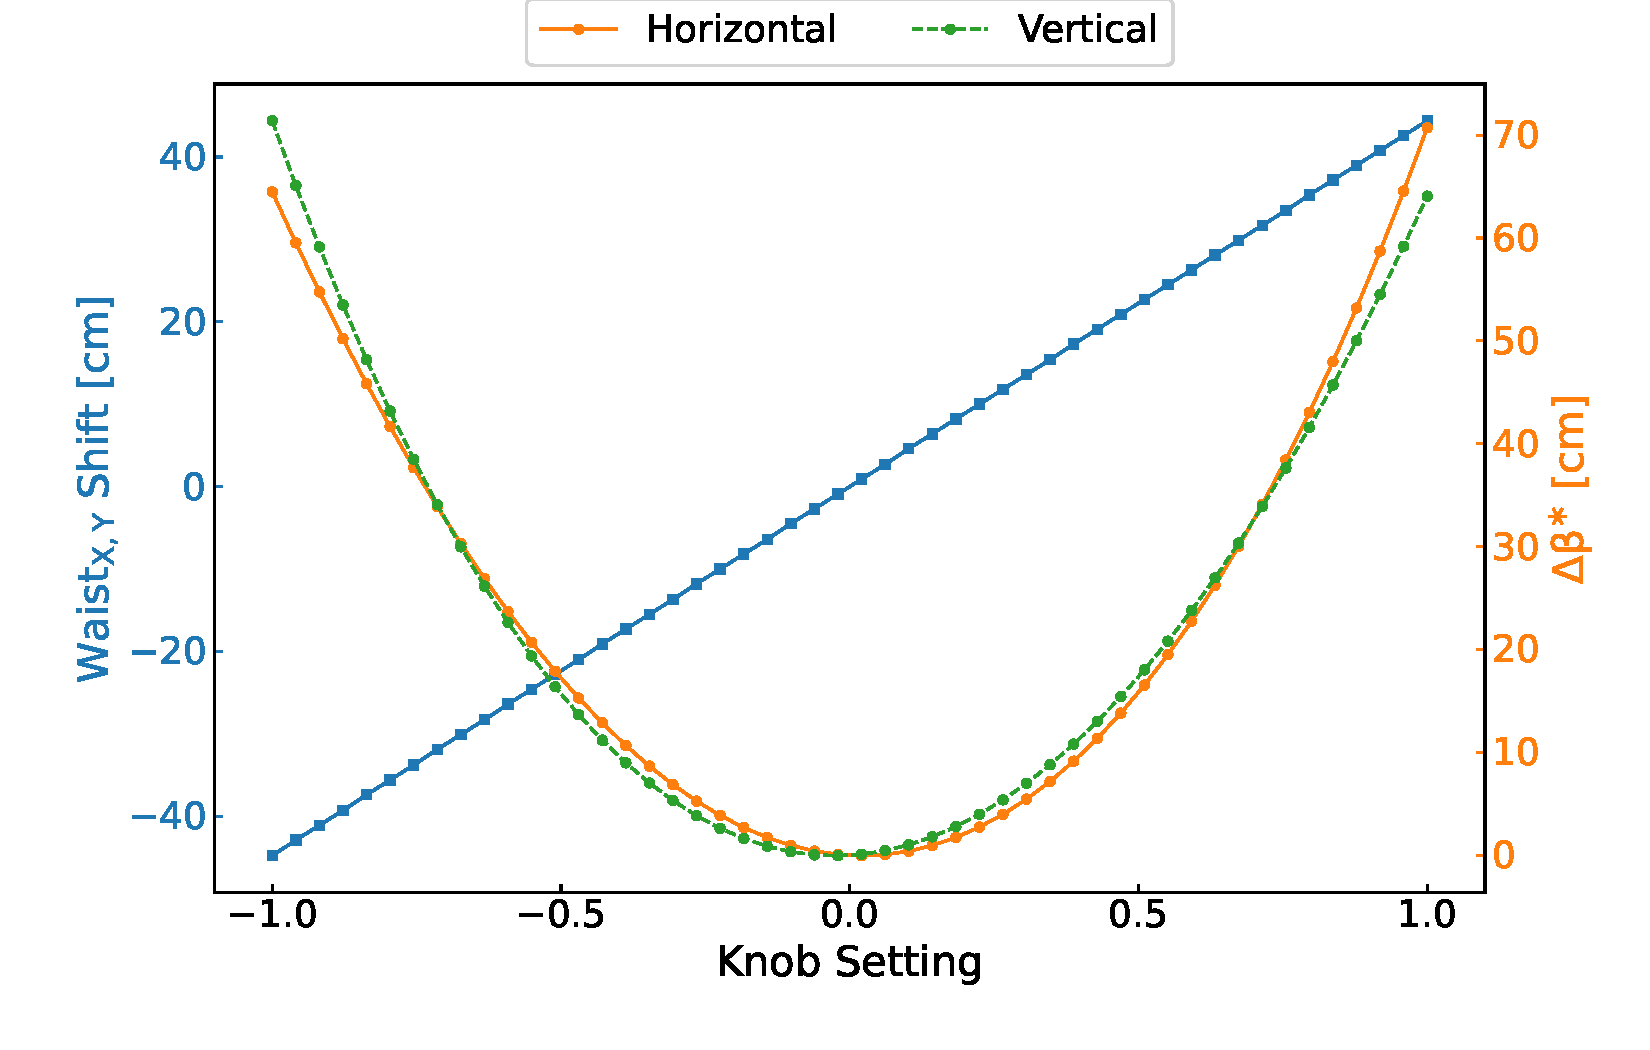
\includegraphics[width=\textwidth]{Figures/IR_Coupling_Correction/rigid_waist_shift_waist_effect_combined.pdf}
    \caption{Simulated effect of the designed Rigid Waist Shift knob as defined in \cref{table:rigid_waist_shift_knob} on the \(\beta^{\ast} =\) \qty{30}{\centi\metre} optics of \num{2022}. The \textcolor{mplblue}{blue} line represents the waist displacement from the design location. The \textcolor{mplorange}{orange} and \textcolor{mplgreen}{green} lines represent the horizontal and vertical \(\beta\)-functions change at the IP as the waist is displaced, respectively.}
    \label{figure:rigid_waist_shift_knob_effect_on_waist}
\end{figure}

The waist displacement from the design location (\textcolor{mplblue}{blue} line) is almost completely linear with the knob setting.
One can note that the minima of the parabolas indicating the change of \(\beta\)-functions at the IP (\textcolor{mplblue}{blue} and \textcolor{mplorange}{orange} curves) are not found at exactly the zero knob setting, which is because the LHC design optics include a very small waist at IP\num{1} and IP\num{5}.

In \cref{figure:rigid_waist_shift_knob_effect_on_betas} one can observe how the \(\beta\)-functions are affected by the application of an RWS, also simulated with the \(\beta^{\ast} =\) \qty{30}{\centi\metre} optics of \num{2022}.
In this simulation the lattice was sliced to improve the resolution of the data points, which explains the smoother lines compared to, for instance, \cref{figure:lhc_ir5_zoomed}.
One can observe how the (anti-)symmetry of the optics in the IR is broken when applying the knob (full vs dashed lines): the horizontal (\textcolor{mplb}{blue}) and vertical (\textcolor{mplr}{red}) \(\beta\)-functions do not mirror each other anymore.
Inset zooms are included around the location of the MQSX magnets (\textcolor{mqsx_green}{green} vertical lines), showing how the horizontal and vertical \(\beta\)-functions are modified in their vicinity.
The purpose of this setup is detailed in \cref{subsection:rws_application_and_simulations}.

\begin{figure}[!htb]
    \centering
    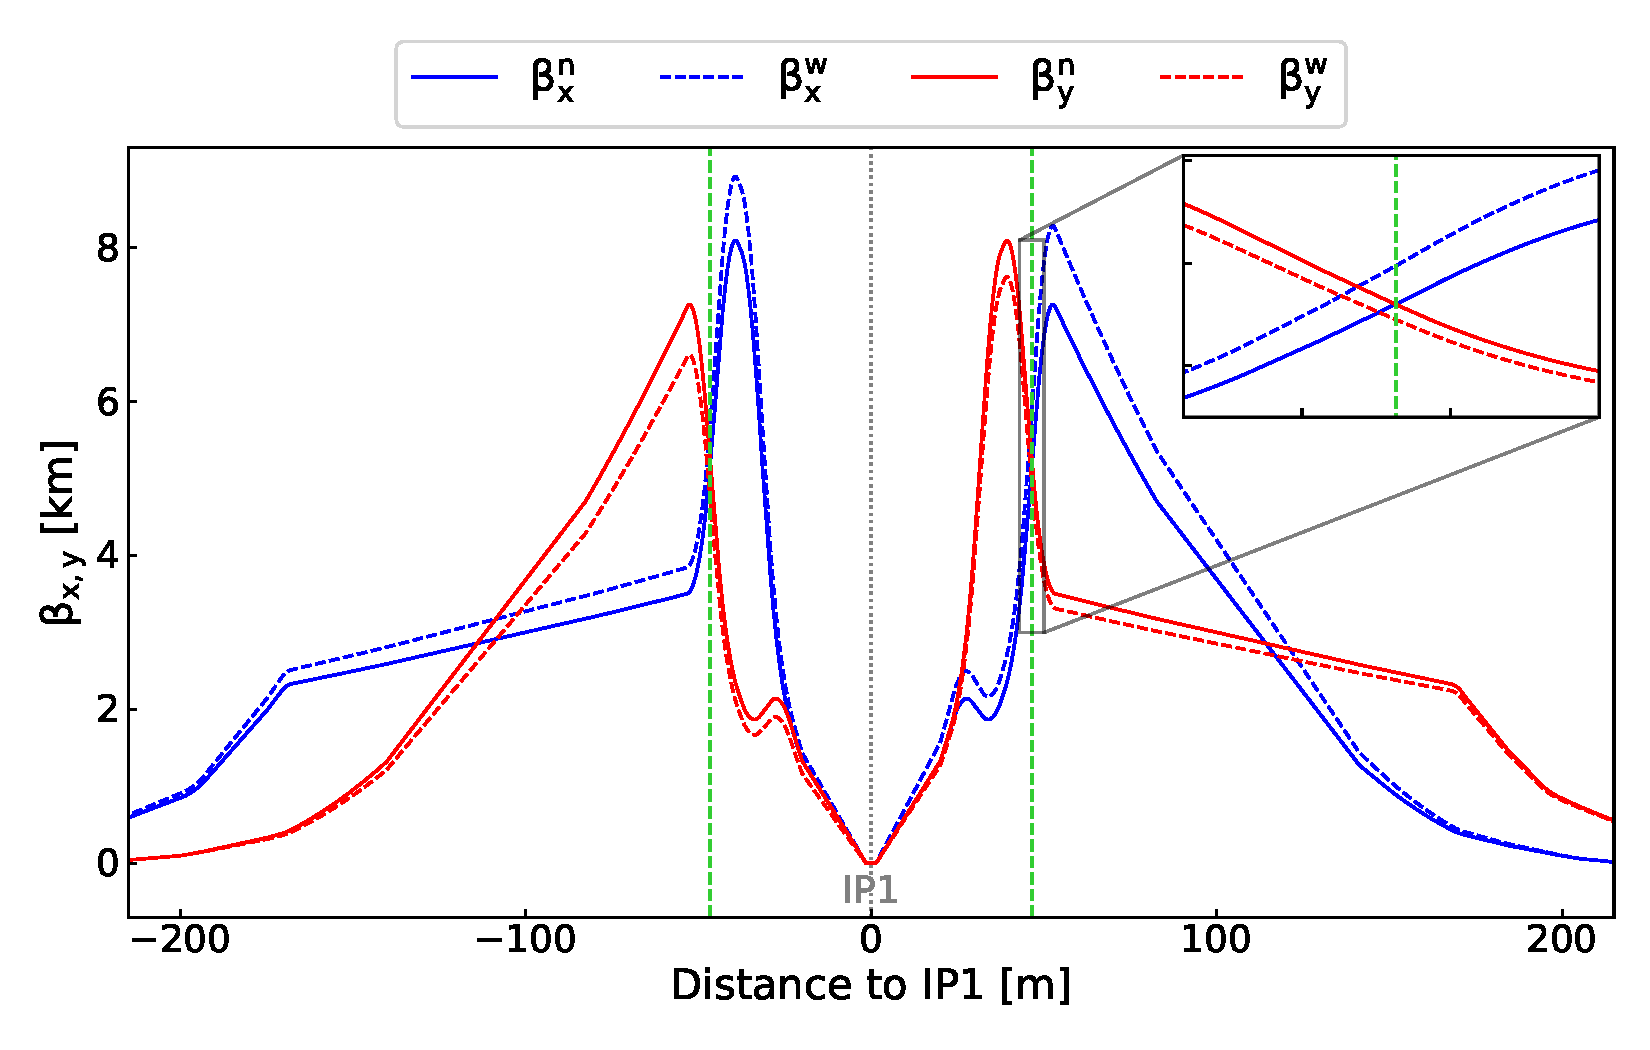
\includegraphics[width=0.99\textwidth]{Figures/IR_Coupling_Correction/rigid_waist_shift_betas_effect.pdf}
    \caption{Simulated effect of the designed RWS knob on the \(\beta\)-functions around IP\num{1}, with the \(\beta^{\ast} =\) \qty{30}{\centi\metre} optics of \num{2022}. The \(\beta\)-functions for both the horizontal (\textcolor{mplb}{blue}) and vertical (\textcolor{mplr}{red}) planes are shown for the nominal (full lines) and shifted waists (dashed lines) scenarios. An identical result is found for IP\num{5}.}
    \label{figure:rigid_waist_shift_knob_effect_on_betas}
\end{figure}

\subsubsection*{Optics Impact and Rematching}

Predictably, the application of an RWS as described above has a strong impact on the optics across the machine: the significant change of \(\beta\)-functions in the triplets sends a beating wave from the IR to the rest of the machine.
Applying an RWS with a unit setting of \num{1}, as defined in \cref{table:rigid_waist_shift_knob}, leads to a \numrange[range-phrase = --]{20}{30}\unit{\percent} increase in \(\beta\)-beating in the machine, depending on the observed beam and plane.

This can be observed in \cref{figure:rigid_waist_shift_betabeating}, where in simulations an RWS was implemented with a unit setting of \num{1} at IP\num{1} and the optics deviations from the nominal scenario were determined across the machine for both beams.
The most affected beam and plane depends on the setting of the RWS: in \cref{figure:rigid_waist_shift_betabeating} beam~\num{1} horizontal and beam~\num{2} vertical are most affected, but these would be beam~\num{1} vertical and beam~\num{2} horizontal if the RWS was applied with a setting of \num{-1}.
Naturally, some strong outliers can be observed in the vicinity of the IP, corresponding to the desired deviation at the IP and in the triplets.

\begin{figure}[!htb]
    \centering
    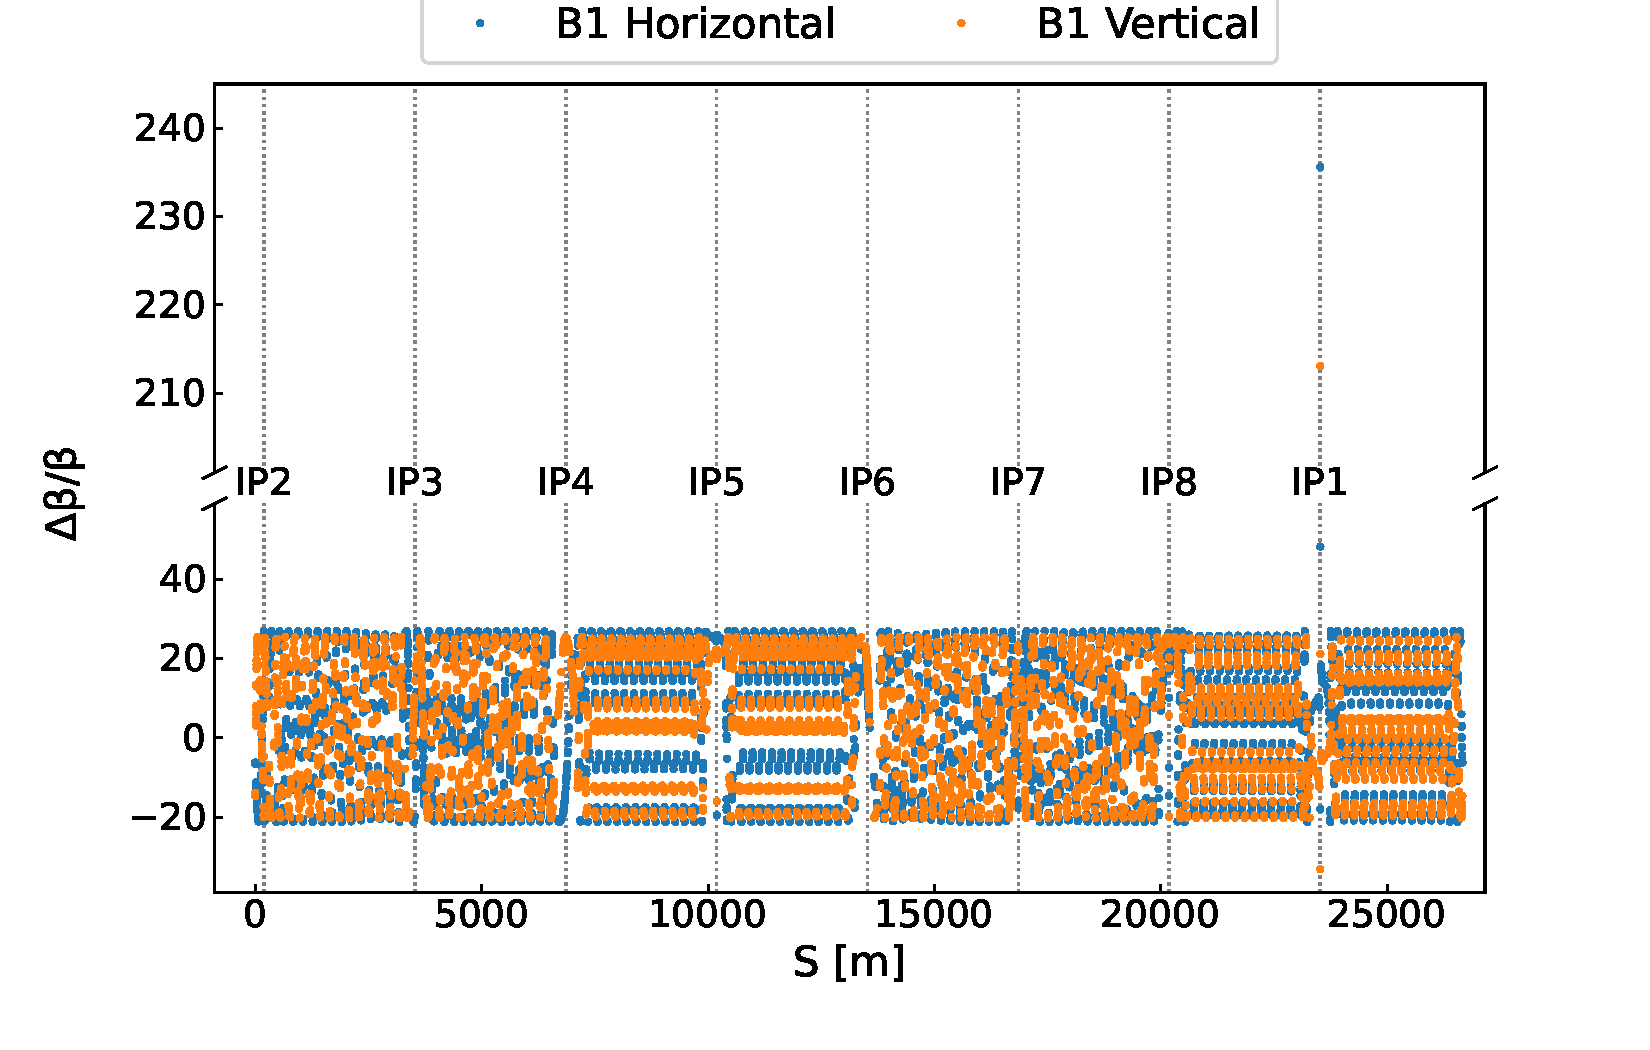
\includegraphics[width=\textwidth]{Figures/IR_Coupling_Correction/rws_ir1_b1_bbeating.pdf}
    \caption{Simulated \(\beta\)-beating induced across beam~\num{1} in both the horizontal (\textcolor{mplblue}{blue}) and vertical (\textcolor{mplorange}{orange}) planes, from applying an RWS as defined in \cref{table:rigid_waist_shift_knob} at IP\num{1}. A \numrange{20}{30}\unit{\percent} \(\beta\)-beating is observed through most of the machine, with (wanted) outliers close to IP\num{1}.}
    \label{figure:rigid_waist_shift_betabeating}
\end{figure}

Such a deviation of the optics has an impact on correction knobs.
For instance, simulations show that application of the RWS causes a \qty{15}{\percent} deviation from the achieved \(\abs{C^{-}}\) to the target value set through the LHC global coupling knobs, used for coupling correction with the arc skew quadrupoles.
Additionally, the optics deviations will change the impact of any errors probed while the RWS is trimmed in, namely the skew quadrupolar impact on the \(\abs{C^{-}}\) (see \cref{equation:deltaqmin_guignard}).
\newline

In order to limit this impact on the optics and guarantee good measurements under an RWS, new correction knobs have been developed that make use of individually powered quadrupoles Q\num{4} to Q\num{10} (included). 
These knobs tune the optics functions and rematch them at the edges of the IR in the large sense.
They were designed with the MAD-X code and a specifically developed Python package that can create these experimental configurations for a given IP in the machine~\cite{CODE:Soubelet:pyrws}.

These knobs are obtained from simulations after applying an RWS in a given IR and iterating several matching routines for quantities of interest at different locations in the machine.
Importantly, no involved magnet sees its powering change by more than \(\sim\)\qty{3}{\percent} with the application of these knobs, which allows for respecting the powering limits of individually powered elements.
As the rematching knobs depend on the RWS setting and optics configuration, many variations are possible and no general definition table is available akin to \cref{table:colinearity_knob,table:rigid_waist_shift_knob}.
A full definition of the rematching knobs for the \(\beta^{\ast} =\)~\qty{30}{\centi\meter} optics of 2022 as implemented and used in the LHC can be found in \cref{section:optics_rematching_knobs_lsa}.

\Cref{figure:rws_rematching_efficiency} shows a comparison of the simulated optics deviation in the beam~\num{1} horizontal plane, induced by the RWS before (\textcolor{mplblue}{blue}) and after (\textcolor{mplorange}{orange}) applying the rematching knob, here implemented at IP\num{1}.
Across the machine the \(\beta\)-beating is brought down by \(\sim\)\qty{20}{\percent} to around \(\sim\)\qty{5}{\percent} depending on the beam and plane compared to the nominal scenario, except for the vicinity of the IP where the wanted deviation is kept.
A \qty{5}{\percent} \(\beta\)-beating across the machine is an acceptable level as it is similar to the level of control achieved during normal operation with all corrections trimmed in, as can be seen in \cref{figure:virgin_vs_corrected_lhcb2}.

While only beam~\num{1} horizontal is shown in this figure, results are similar for all planes of beam~\num{1} and beam~\num{2}.
As the rematching depends on the desired configuration (given optics and setting of the RWS) a knob has to be designed for each beam, at each IR and for each RWS setting.

\begin{figure}[!htb]
    \centering
    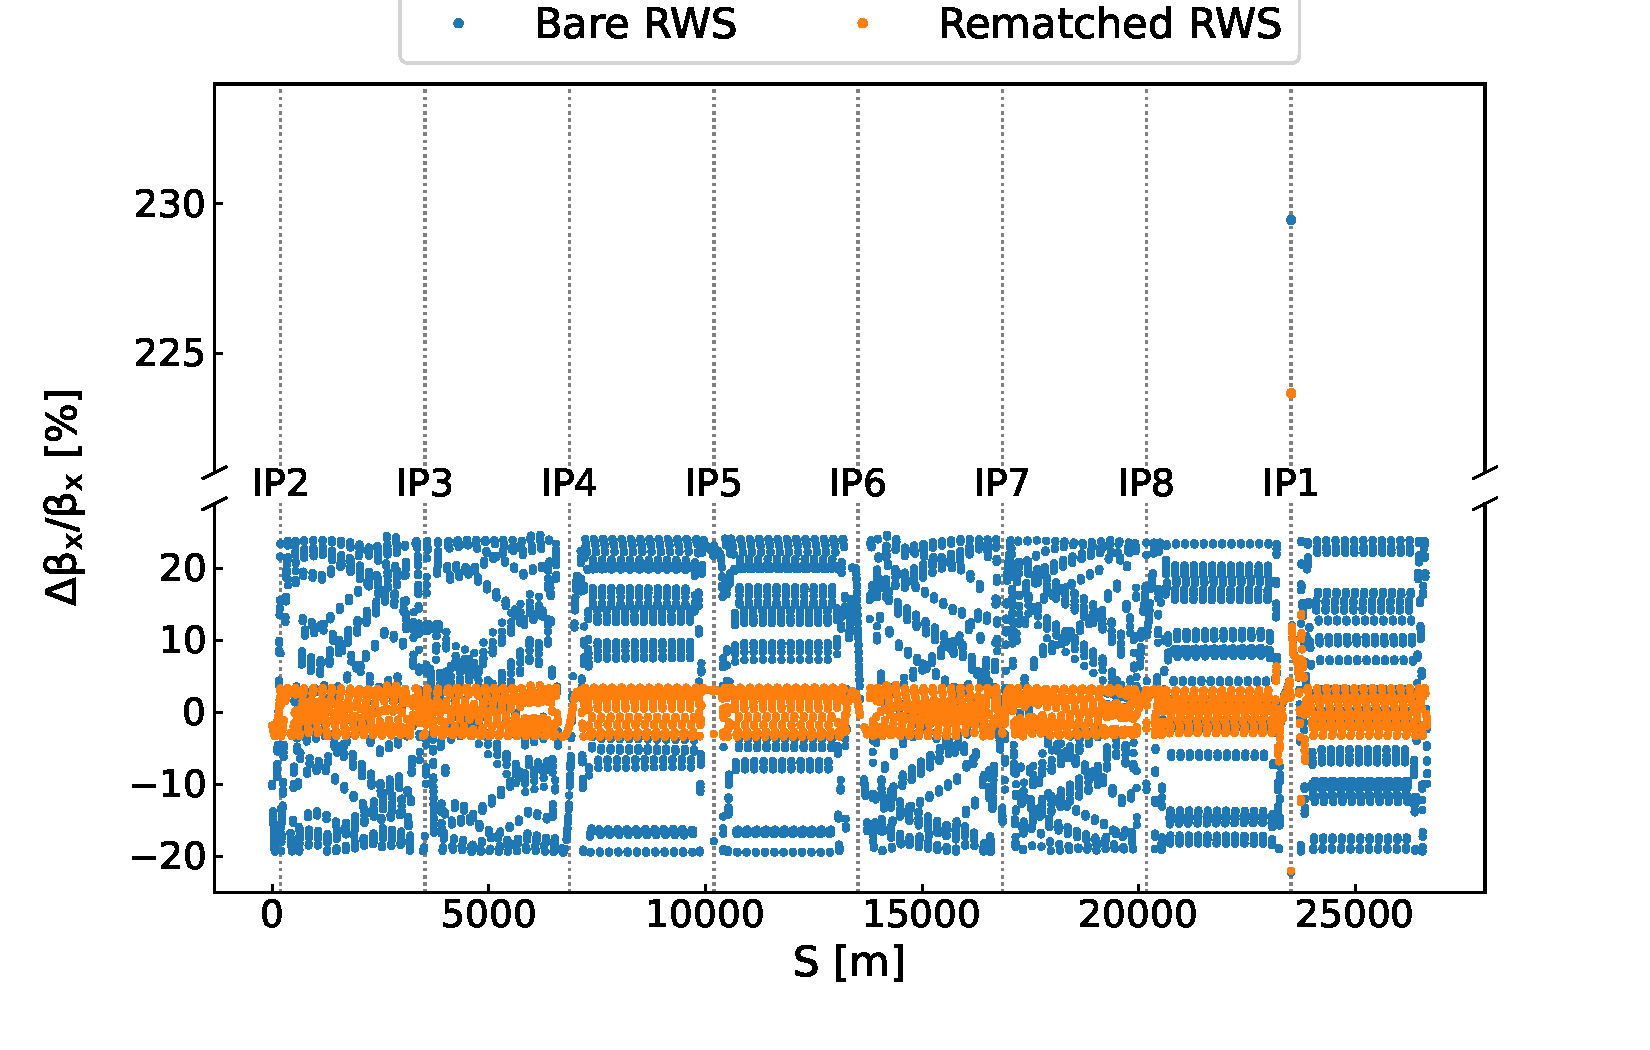
\includegraphics[width=\textwidth]{Figures/IR_Coupling_Correction/rws_ir1_b1_bbeating_rematched.pdf}
    \caption{Simulated \(\beta\)-beating induced across the machine in the beam~\num{1} horizontal plane from applying an RWS at IP\num{1}, before (\textcolor{mplblue}{blue}) and after (\textcolor{mplorange}{orange}) applying the optics rematching knob.}
    \label{figure:rws_rematching_efficiency}
\end{figure}

One can notice that near the IP the beating is also lowered by the rematching, but stays high enough to still break the symmetry of the IR.
\Cref{figure:rws_ir1_rematching_betas} shows the \(\beta\)-functions around IP\num{1} before (full lines) and after (dashed lines) application of the rematching knobs.
One can observe how the deviation between the two cases is negligible and, importantly, in both cases the symmetry of the IR is broken compared to, for instance, \cref{figure:lhc_ir5_zoomed}.
\todo{need about make two lines of content here at some point, so I push section 1.4.2 down below the figure I'm talking about, which really helps the readability.}

\begin{figure}[!htb]
    \centering
    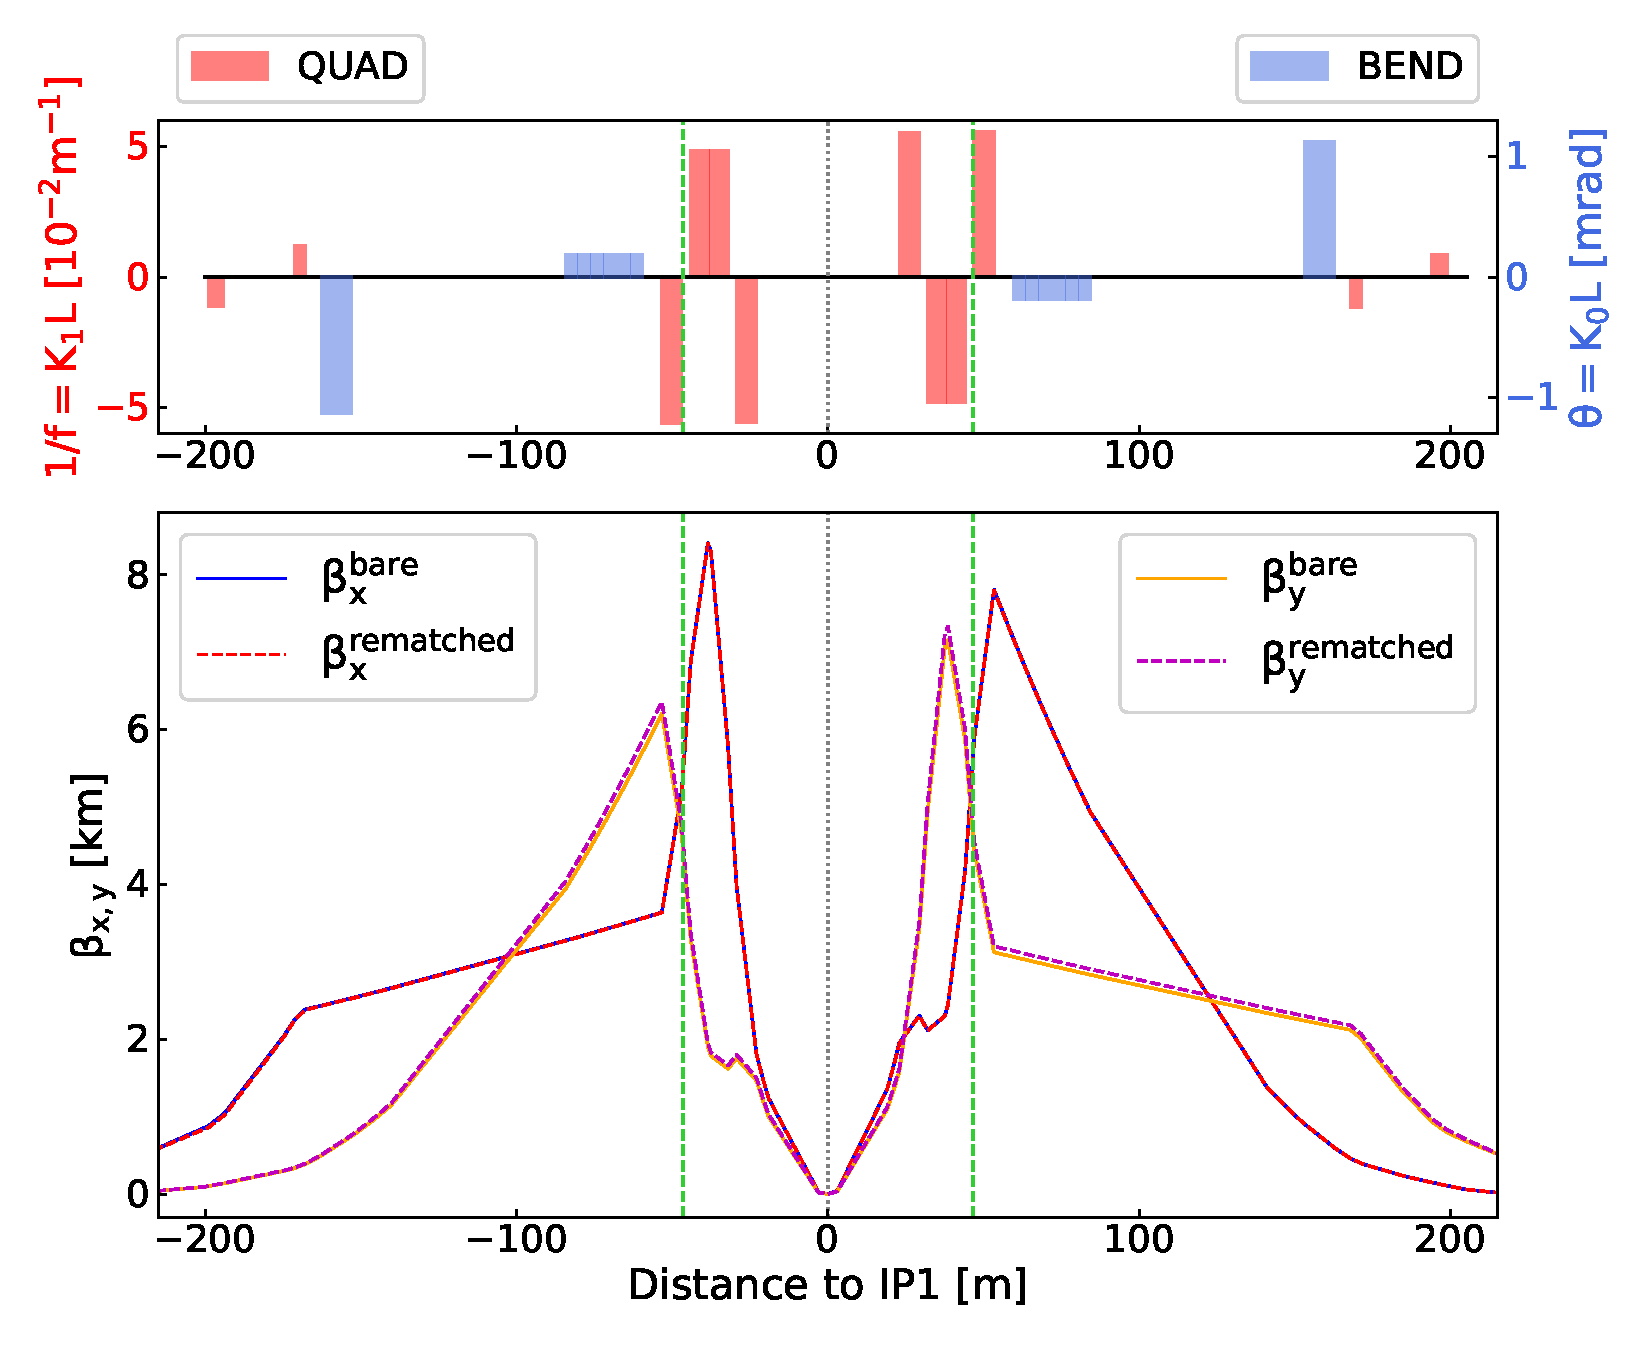
\includegraphics[width=0.95\textwidth]{Figures/IR_Coupling_Correction/rws_ir1_rematching.pdf}
    \caption{Simulated \(\beta\)-functions around IP\num{1} when applying an RWS, before (full lines) and after (dashed lines) application of the rematching knobs, with the \(\beta^{\ast} =\) \qty{30}{\centi\metre} optics of \num{2022}.}
    \label{figure:rws_ir1_rematching_betas}
\end{figure}

\subsection{Application Concept and Simulations}
\label{subsection:rws_application_and_simulations}

Making away with the optics symmetry of the IR allows to break the locality of any coupling bump, even a truly local one.
As can be seen on the inset zooms of \cref{figure:rigid_waist_shift_knob_effect_on_betas}, with the application of an RWS the \(\beta\)-functions at the MQSX magnets change enough that the \(\sqrt{\beta_x \beta_y}\) term in \cref{equation:deltaqmin_only_mqsxs} are different at the two magnets.
\Cref{table:sqrt_betas_from_rws} shows the values of these terms with and without an RWS applied.
Phase advances are also changed, but by a very small amount.

\begin{table}[!htb]
    \centering
    \begin{tblr}{colspec={ccc}}
        \hline
        \SetCell[r=2,c=1]{m,c} \textbf{Magnet} & \SetCell[c=2]{c} \textbf{\(\sqrt{\beta_x \beta_y}\) [\unit{\square\meter}]}   \\
        \cline{2,3}                            &  Without an RWS            &    With an RWS                                   \\
        \hline
        MQSX.3L[IP]                            &    \num{5193.084265}       &     \num{5186.603944}                            \\
        MQSX.3R[IP]                            &    \num{5199.142377}       &     \num{5396.527580}                            \\
        \hline
    \end{tblr}
    \caption{Values of the \(\sqrt{\beta_x \beta_y}\) term in \cref{equation:deltaqmin_only_mqsxs} at the MQSX magnets around IP\num{1} or IP\num{5} without (left) and with (right) the application of an RWS, with the \(\beta^{\ast} =\) \qty{30}{\centi\metre} optics of \num{2022}.}
    \label{table:sqrt_betas_from_rws}
\end{table}

\Cref{figure:rdt_leak} shows the coupling RDTs from a closed coupling bump around the IP created through the colinearity knob, both in the presence (\textcolor{mplr}{red}) and absence (\textcolor{mplb}{blue}) of an RWS.

\begin{figure}[!htb]
    \centering
    \includegraphics*[width=\textwidth]{Figures/IR_Coupling_Correction/waist_shift_leaks_rdts.pdf}
    \caption{Amplitudes of the linear coupling RDTs in the vicinity of IP\num{1} under a coupling bump, with (\textcolor{mplr}{red}) and without (\textcolor{mplb}{blue}) an RWS. The vertical \textcolor{mqsx_green}{green} lines represent the positions of the skew quadrupoles correctors (MQSX.\num{3}[RL]\num{1}) used to implement the coupling bump. A colinearity knob setting of \num{10} and a rigidity waist shift knob setting of \num{1} were used.}
    \label{figure:rdt_leak}
\end{figure}

When applying a Rigid Waist Shift and breaking the optics symmetry of the IR, on can observe a leakage of the coupling RDTs outside the limits of the initial coupling bump.
These RDTs will then have a residual presence in the machine, which can be measured and reconstructed from turn-by-turn data from BPMs with more suitable phase advances.
As a consequence, under an RWS even a local coupling bump that would normally be invisible to the rest of the machine will have a direct impact on the global coupling, measured as the \(\abs{C^{-}}\).

This can be seen in \cref{figure:knob_to_cminus_with_waist}, where changes in the setting of the colinearity knob now have a strong effect on the \(\abs{C^{-}}\) when an RWS is applied in the machine.

\begin{figure}[!htb]
    \centering
    \includegraphics*[width=0.99\textwidth]{Figures/IR_Coupling_Correction/colin_knob_vs_waist_shift.pdf}
    \caption{Impact of the colinearity knob on the global \(\abs{C^{-}}\), calculated according to \cref{equation:deltaqmin_from_f1001}, with (\textcolor{mplorange}{orange}) and without (\textcolor{mplblue}{blue}) applying an RWS.}
    \label{figure:knob_to_cminus_with_waist}
\end{figure}

As previously mentioned, since the bump is not actually perfectly closed the (\textcolor{mplorange}{orange}) line in \cref{figure:knob_to_cminus_with_waist} is not completely flat and reaches up to \(\sim\)~\num{1e-5}, which is well below the measurement accuracy for the \(\abs{C^{-}}\).
The behavior seen in \cref{figure:knob_to_cminus_with_waist}, though theoretical, has been experimentally tested and confirmed in the machine~\cite{CERN:Persson:Local_Coupling_IP}.
Importantly, this behavior opens the possibility of using an RWS to probe IR local coupling through the measured global coupling.
\newline

Simulations have been done to investigate the feasibility of finding local coupling correction settings using an RWS, using the \(\beta^{\ast} = \) \qty{30}{cm} optics of \num{2022}.
At both IR\num{1} and IR\num{5} a local coupling bump was created by introducing identical tilt errors in triplet quadrupoles Q\num{3} - thus giving a skew quadrupolar component - and the colinearity knob was powered for compensation.
A full parameter space was explored, both with and without an RWS applied.
\Cref{figure:cminus_colin_vs_tilt_with_waist} shows the values of the resulting \(\abs{C^{-}}\) across the parameter space when an RWS is applied.

\begin{figure}[!htb]
    \centering
    \includegraphics*[width=0.91\textwidth]{Figures/IR_Coupling_Correction/cminus_colin_tilt_compensation_with_waist.pdf}
    \caption{Resulting \(\abs{C^{-}}\) (\cref{equation:deltaqmin_from_f1001}) for various combinations of tilt error and colinearity knob settings, when applying an RWS.}
    \label{figure:cminus_colin_vs_tilt_with_waist}
\end{figure}

\Cref{figure:beam_size_colin_vs_tilt_no_waist} shows the resulting beam size increase as a ratio to the nominal beam size across the same parameter space.

\begin{figure}[!htb]
    \centering
    \includegraphics*[width=0.91\textwidth]{Figures/IR_Coupling_Correction/ip_beam_size_growth_colin_tilt_compensation_no_waist.pdf}
    \caption{Resulting beam size (\cref{equation:lebedev_beam_size}) increase for identical settings of tilt error and colinearity knob settings as \cref{figure:cminus_colin_vs_tilt_with_waist}, but without an RWS.}
    \label{figure:beam_size_colin_vs_tilt_no_waist}
\end{figure}

The results of \cref{figure:beam_size_colin_vs_tilt_no_waist} highlight that minimization of the growth is possible though a wrong setting would enhance the phenomenon.
A great correlation between beam size growth from the local coupling bump (without RWS) and the \(\abs{C^{-}}\) from leaked RDTs (with RWS) is observed, which is an encouraging first result.
\newline

Simulations replicating a more complex scenario - akin to operational conditions - were also performed.
In these, tilt errors were introduced in triplet quadrupoles Q\num{3} as previously to create a closed local coupling bump around the IP.
Additionally, some tilt errors were added to an individually powered quadrupole in IR\num{5} (for instance Q\num{5}) to include the presence of expected residual local coupling errors in the other main IR, which contribute to the global coupling by the amount of \num{1e-3}.
Some global coupling sources were also added with a dedicated knob~\cite{CERN:Tomas:Optimizing_Global_Coupling_Knobs_LHC} that bring the global coupling to \num{1e-2}, which was then corrected through a routine and brought down to \(\sim\)\num{3e-3}, a level similar to what is achieved in the machine~\cite{PRES:Persson:Transverse_Coupling_OMC_OP,PRES:Persson:Transverse_Coupling_Stability_HLLHC_WP2}.
The RWS and colinearity knobs were then powered to different settings, and the resulting \(\abs{C^{-}}\) and IP beam sizes were determined in all settings combinations.

Similar to the previous studies made for \cref{figure:cminus_colin_vs_tilt_with_waist,figure:beam_size_colin_vs_tilt_no_waist}, an entire parameter space of implemented errors and corrections has been explored.
The evolution of both the \(\abs{C^{-}}\) and the beam size growth at IP\num{1} for one of these simulations can be seen in \cref{figure:full_scenario_colin_correction_dqmin_lebedev}.
These curves would correspond to a vertical line in \cref{figure:cminus_colin_vs_tilt_with_waist,figure:beam_size_colin_vs_tilt_no_waist}, but with a realistic scenario.

\begin{figure}[!htb]
    \centering
    \includegraphics*[width=\textwidth]{Figures/IR_Coupling_Correction/full_scenario_cminus_and_ip_size.pdf}
    \caption{Resulting \(\abs{C^{-}}\) (\cref{equation:deltaqmin_from_f1001}) under an RWS (\textcolor{mplorange}{orange}) and IP\num{1} beam size (\cref{equation:lebedev_beam_size}) without an RWS relative to the nominal scenario (\textcolor{mplblue}{blue}), for various colinearity knob settings. The black dotted line represents the threshold of a \qty{1}{\percent} beam size increase from the nominal scenario.}
    \label{figure:full_scenario_colin_correction_dqmin_lebedev}
\end{figure}

It can be observed that settings minimizing the measured \(\abs{C^{-}}\) under an RWS are very close to minimizing the coupling induced beam size increase without said RWS.
In this case, these settings also compensate for the contribution of the other added sources to the global coupling, on top of the local ones.
Similarly to previous studies a great correlation is observed, and across the parameter space one computes a \num{0.96} Pearson correlation coefficient between the two quantities shown in \cref{figure:full_scenario_colin_correction_dqmin_lebedev}.
This confirms the link between the measured \(\abs{C^{-}}\) and the quantities of interest at the IP location.
To summarize:
\begin{itemize}
    \item Thanks to the RWS, truly local errors can be probed through their forced impact on global coupling.
    \item Using the correlation properties demonstrated above, one can find settings to minimize the coupling and its effects at the IP.
\end{itemize}

\subsection{Determining Corrections}

The corrections which would compensate only the local sources are determined by comparing the measured \(\abs{C^{-}}\) to simulations, such as the orange line in \cref{figure:full_scenario_colin_correction_dqmin_lebedev}.

In the real machine, some coupling will remain in the arcs due to a non-perfect global correction and non-local SbS corrections.
As the method probes local errors' impact through the \(\abs{C^{-}}\), it will naturally be sensitive to the global coupling in the machine, which should be replicated in simulations.
Although the overall behavior of simulations remains similar when including this component, an important change from the line seen in \cref{figure:full_scenario_colin_correction_dqmin_lebedev} is the location of the setting that minimizes the \(\abs{C^{-}}\).
The relevance of this property will be discussed below.
By comparing measurements from a colinearity knob scan to simulations - where the former includes the impact of local errors, but the latter does not - one can single out the contribution of the local sources to global coupling.

\begin{figure}[!htb]
    \centering
    \includegraphics*[width=0.95\textwidth]{Figures/IR_Coupling_Correction/full_scenario_determine_correction.pdf}
    \caption{Resulting \(\abs{C^{-}}\) in simulations as done for \cref{figure:full_scenario_colin_correction_dqmin_lebedev}, with (\textcolor{mplblue}{blue}) and without (\textcolor{mplorange}{orange}) local coupling sources in IR\num{1}.}
    \label{figure:full_scenario_determine_correction}
\end{figure}

\Cref{figure:full_scenario_determine_correction} shows the resulting \(\abs{C^{-}}\) values under an RWS during a colinearity knob scan, for one of the simulation scenarios mentioned previously (\cref{figure:full_scenario_colin_correction_dqmin_lebedev}) (\textcolor{mplblue}{blue}), and a similar scenario in which no local coupling sources were implemented in IR\num{1} (\textcolor{mplorange}{orange}).
The former represents what would be measured in the machine, including the contribution of local sources.
The latter represents a simulation to compare such a measurement to, which includes all contributions to global coupling except for the IR local sources.
The highlighted difference between the two curves is then fully explained by the local sources.

Applying a trim of the colinearity knob setting linearly translates the curves of \cref{figure:full_scenario_determine_correction} horizontally.
This behavior is valid and verifiable in both simulation and measurements.
Therefore, one looks to determine a colinearity knob trim that, if applied in the machine, would bring the measurement's \(\abs{C^{-}}\) minimization point to that of the simulation.

\begin{figure}[!htb]
    \centering
    \includegraphics*[width=0.95\textwidth]{Figures/IR_Coupling_Correction/full_scenario_correction_efficiency.pdf}
    \caption{Relative IP beam sizes when compared to the nominal scenario (\textcolor{mplblue}{blue}) when inputting the local errors used in the study for \cref{figure:full_scenario_determine_correction} (\textcolor{mplorange}{orange}) and after applying the suggested correction (\textcolor{mplgreen}{green}). The black dotted line represents the threshold of a \qty{1}{\percent} beam size increase from the nominal scenario.}
    \label{figure:full_scenario_correction_efficiency}
\end{figure}

As this difference if fully explained by local sources, this trim contains the information on the local error in terms of colinearity knob setting: powering of the corrector magnets.
In \cref{figure:full_scenario_determine_correction} the minima are highlighted with vertical lines and the aforementioned correction trim is determined from the relative position of these two minima.
The value is different from that of the minimization in \cref{figure:full_scenario_colin_correction_dqmin_lebedev} as there global sources are also compensated while this correction aims at compensating only the local sources.

When only considering the local sources used for the results in \cref{figure:full_scenario_determine_correction} and inputting the correction trim suggested, one obtains a good compensation of the beam sizes at IP\num{1}.
\Cref{figure:full_scenario_correction_efficiency} shows the impact of these local errors and the effect of applying the suggested correction trim.
The exactitude and effectiveness of the determined correction can be improved by performing more granular scans of the colinearity knob, but the values used are representative of what can be done in measurements.

\subsubsection*{Reproducing the Machine's Coupling}

The reproduction of the machine's global coupling in simulations becomes necessary as soon as strong non-IR sources are present.
This reproduction can be done in different ways.
In studies, various implementations were tested: random tilts in all quadrupoles, LHC specific knobs~\cite{CERN:Tomas:Optimizing_Global_Coupling_Knobs_LHC}, longitudinal misalignment of sextupoles, field errors in specific magnets or random combinations of the above.
These can be seen in \cref{figure:global_coupling_modeling_impact} where for each scenario the minimization point is highlighted by a vertical dashed line.

\begin{figure}[!hbt]
    \centering
    \includegraphics*[width=\textwidth]{Figures/IR_Coupling_Correction/global_sources_influence.pdf}
    \caption{Resulting simulated \(\abs{C^{-}}\) under an RWS during a scan of the colinearity knob, for various implementations of global coupling in the machine. For each case a vertical dashed line highlights the location of the minimization point.}
    \label{figure:global_coupling_modeling_impact}
\end{figure}

In all investigated scenarios the achieved \(\abs{C^{-}}\) before applying the RWS is the same value before (\(\sim 10^{-2}\)) and after (\(\sim 2 \cdot 10^{-3}\)) applying a correction routine.
It was found that, to the levels of coupling we achieve after correcting the machine the distribution and implementation of sources had little impact on the minimization point of the \(\abs{C^{-}}\) curve under and RWS, as long as the overall pattern of the \(f_{1001}\) and the level of coupling measured in the machine were accurately reproduced.
One can see in \cref{figure:global_coupling_modeling_impact} how the minimization point is relatively unchanged by the global coupling implementation method within the precision of the mesh step used for the scan, which was chosen to reflect that achievable in the machine.
As a consequence, in simulations this reproduction was done by including the coupling correction knobs implemented in the machine, as determined during earlier commissioning steps.

\subsection{Rigid Waist Shift Procedure}

To summarize so far, two tools are now available to tackle local coupling correction:
\begin{itemize}
    \item The colinearity knob (\cref{table:colinearity_knob}) allows adjusting the coupling at the IP without affecting the rest of the machine, namely previously established corrections.
    \item The rigid waist shift knob (\cref{table:rigid_waist_shift_knob}) allows probing local errors through the \(\abs{C^{-}}\) (\cref{figure:rdt_leak,figure:knob_to_cminus_with_waist}) and to find a correction setting of the colinearity knob that will minimize the coupling at the IP (\cref{figure:full_scenario_determine_correction,figure:full_scenario_correction_efficiency}).
\end{itemize}

Using those, the complete correction procedure for local linear coupling is then made of three steps:
\begin{enumerate}
    \item Firstly, calculating and applying a correction of the IR contribution to global coupling based on RDTs from turn-by-turn measurements, using the SbS technique.
    \item Secondly, breaking the optics symmetry between the right and left-hand side of the IP by applying an RWS, and performing a scan of the colinearity knob.
    \item Finally, analyzing the measurements data and comparing it to simulations in order to find a colinearity knob adjustment setting that minimizes the global coupling, without impacting the correction found in step~\num{1}.
\end{enumerate}

These measurements can be performed for each IR and for each beam, and the subsequent determined corrections can then be directly applied in the machine.

%----------------------------------------------------------------------------------------

\section{Local Coupling Correction in the LHC 2022 Commissioning}
\label{section:rws_experimental_results}

Below are presented experimental results of local coupling correction in the LHC's first year of Run~\num{3}, using the RWS procedure of this chapter.
One can refer to \Cref{appendix:experimental_knobs} for information on the fills used for experimental measurements.

\subsection{Segment-by-Segment Corrections}

In October \num{2021} a week of beam tests was done in the LHC at injection energy.
From the measurements at \qty{450}{\giga\electronvolt} a first set of local coupling corrections were calculated for each of the four main IRs using the segment-by-segment technique.
\Cref{figure:beam_test_sbs_abs_f1001_ip5} shows the segment-by-segment results for the absolute value of the \(f_{1001}\) RDT in IR\num{5}, from the \num{12}\({}^\mathrm{th}\) BPM left to right of IP\num{5}.
The vertical gray line indicates the location of the IP in the segment.
Due to the skew quadrupole correctors in the IRs being single aperture magnets, one needs to find a single powering setting that works for both beams and both are shown on the figure.

\begin{figure}[!htb]
    \centering
    \includegraphics*[width=\textwidth]{Figures/IR_Coupling_Correction/beamtest_sbs_abs_f1001_ip5.pdf}
    \caption{Propagation of the measured \(\abs{f_{1001}}\) around IP\num{5} (dashed gray line) and of the reconstructed values from the determined correction, measured at \qty{450}{\giga\electronvolt} and \(\beta^{*}=\) \qty{11}{\meter}.}
    \label{figure:beam_test_sbs_abs_f1001_ip5}
\end{figure}

One can see that the determined correction in IR\num{5} matches the propagated measurement within the tolerance of the error bars at the edges of the segment.
This guarantees a good compensation of the IR's contribution to global coupling.

During the LHC Run~\num{3} commissioning, local coupling corrections determined during the previous year's beam test were trimmed in the machine from the start.
After reaching the \(\beta^{*}=\) \qty{30}{\centi\meter} optics, where the machine is more sensitive to local errors, a noticeable deviation around IP\num{1} was observed and a refinement of the correction was determined, still with the segment-by-segment technique.
\Cref{figure:commissioning_sbs_real_f1001_ip1,,figure:commissioning_sbs_imag_f1001_ip1} show the effect of the new correction on the real and imaginary parts of the \(f_{1001}\) RDT in the segment, respectively.

\begin{figure}[!htb]
    \centering
    \includegraphics*[width=\textwidth]{Figures/IR_Coupling_Correction/commissioning_sbs_real_f1001_ip1.pdf}
    \caption{Propagation of the measured \(\Re f_{1001}\) around IP\num{1} (dashed gray line) and the reconstructed values from the determined correction, measured at \qty{6.8}{\tera\electronvolt} and \(\beta^{*}=\) \qty{30}{\centi\meter}.}
    \label{figure:commissioning_sbs_real_f1001_ip1}
\end{figure}
  
\begin{figure}[!htb]
    \centering
    \includegraphics*[width=\textwidth]{Figures/IR_Coupling_Correction/commissioning_sbs_imag_f1001_ip1.pdf}
    \caption{Propagation of the measured \(\Im f_{1001}\) around IP\num{1} (dashed gray line) and the reconstructed values from the determined correction, measured at \qty{6.8}{\tera\electronvolt} and \(\beta^{*}=\) \qty{30}{\centi\meter}.}
    \label{figure:commissioning_sbs_imag_f1001_ip1}
\end{figure}

The beating observed from the old correction was re-matched thanks to a new corrector setting where the IR\num{1} right-hand side corrector's powering was changed by \qty{1e-4}{\per\square\meter}.
The correction settings determined with the segment-by-segment technique and trimmed in the machine at the four main IRs can be found in \cref{table:sbs_corrections}, as well as their counterpart values from Run~\num{2}.

\begin{table}[!htb]
    \centering
    \begin{tblr}{colspec={ccc}}
        \hline
        \SetCell[c=1]{c} \textbf{Circuit} & \SetCell[c=2]{c} \textbf{\( \Delta k \)~[\qty{1e-4}{\per\square\meter}]}              \\
        \cline{2,3}
                                 &    \textbf{2016-2018}~\cite{CERN:Persson:LHCOpticsCorrectionsEvian2019}    &    \textbf{2022}  \\
        \hline
            \textbf{RQXS.3L1}    &    \num{11}                                                                &     \num{8}       \\
            \textbf{RQXS.3R1}    &    \num{7}                                                                 &     \num{7}       \\
            \hline[dashed]
            \textbf{RQXS.3L2}    &    \num{-14}                                                               &     \num{-14}     \\
            \textbf{RQXS.3R2}    &    \num{-14}                                                               &     \num{-14}     \\
            \hline[dashed]
            \textbf{RQXS.3L5}    &    \num{7}                                                                 &     \num{6}       \\
            \textbf{RQXS.3R5}    &    \num{7}                                                                 &     \num{6}       \\
            \hline[dashed]
            \textbf{RQXS.3L8}    &    \num{-5}                                                                &     \num{-5}      \\
            \textbf{RQXS.3R8}    &    \num{-5}                                                                &     \num{-5}      \\
        \hline
    \end{tblr}
    \caption{Skew quadrupole correctors' powering at the four main LHC IRs as determined with the segment-by-segment technique, in \num{2022} (right) compared to their values used during Run~\num{2} (left).}
    \label{table:sbs_corrections}
\end{table}

\subsection{Rigid Waist Shift }

\subsection{Luminosity Confirmation}

\begin{table}[!htb]
    \centering
    \begin{tblr}{colspec={ccc}}
        \hline
        \SetCell[r=2,c=1]{m,c} \textbf{Experiment} & \SetCell[c=2]{c} \textbf{Luminosity Gain [\unit{\percent}]}                     \\
        \cline{2,3}                                &    \(\beta^{\ast} = \) \qty{30}{cm}    &    \(\beta^{\ast} = \) \qty{42}{cm}    \\
        \hline
        \textbf{ATLAS (IP\num{1})}                 &    \num{9.7}                           &     \num{5.2}                          \\
        \textbf{CMS (IP\num{5})}                   &    \num{3.5}                           &     \num{1.5}                          \\
        \hline
    \end{tblr}
    \caption{Luminosity gains observed at the main experiments ATLAS and CMS from the method's suggested corrections.}
    \label{table:rws_lumi_gains}
\end{table}


\subsection{Inconclusive Measurements}

\todo{Talk about the negative RWS measurements that turned out trash because they gave non-trustworthy corrections suggestions.}

\section{Operation with Limited Correctors Availability}
\label{section:limited_correctors_availability}

Mitigation Options in Case of MQSX Failures
\todo{Uncomment text when I get here, take mostly the structure of the IPAC23 article and project update V. Go deeper in details (see commented out subsections).}

% \subsection{Lifetime Considerations of MQSX Elements}

% Explain that there is a real risk that some of our MQSX magnets die, especially the ones in IR1 (ATLAS).
% In this case, we will need a containment plan, as not only are they used for the but the local corrections they are a part of are a baseline for us to compute higher order terms corrections.

% \Cref{table:correctors_peak_dose} reproduced from slide 23~\cite{Evian21:Cerutti:TripletLifetime}:

% \begin{table}[!htb]
%     \centering
%     \caption{Expected total received dose of the corrector magnets located in the triplets for the main IRs. Table reproduced from~\cite{Evian21:Cerutti:TripletLifetime}. The entries marked with \asterisk assume an IR\num{1} polarity inversion in the middle of \num{2025}.}
%     \begin{tblr}{colspec={ccc}}
%         \hline
%         \SetCell[r=3,c=1]{m,c} \textbf{Magnets}             &  \SetCell[c=2]{c} \textbf{Peak Dose [\unit{\mega\gray}]}                                                                                     \\
%         \cline{2,3}                                         &  With ATLAS Variable (Fixed) Angle                        &    +\num{2025} (as \num{2023}/\num{2024})                                        \\
%         \cline{2,3}                                         &  After \qty{395}{\femto\barn^{-1}}                        &    After \qty{480}{\femto\barn^{-1}}                                             \\
%         \hline
%         \textcolor{red}{\textbf{MCBX\num{1} (IR\num{1})}}   &    \textcolor{red}{\num{8.5} (\num{8.5})}                 &     \textcolor{red}{\num{11} (\num{11}) $/$ \asterisk \num{10.5} (\num{10.5})}   \\
%         \textcolor{red}{\textbf{MCBX\num{1} (IR\num{5})}}   &    \num{6}                                                &     \textcolor{red}{\num{7.5}}                                                   \\
%         \textbf{MCBX\num{2} (IR\num{1})}                    &    \num{3.5} (\num{3.5})                                  &     \num{4} (\num{4}) $/$ \asterisk \num{4} (\num{4})                            \\
%         \textbf{MCBX\num{2} (IR\num{5})}                    &    \num{2}                                                &     \num{2.5}                                                                    \\
%         \textcolor{red}{\textbf{MQSX (IR\num{1})}}          &    \textcolor{red}{\num{7.5} (\num{7.5})}                 &     \textcolor{red}{\num{9} (\num{9}) $/$ \asterisk \num{9} (\num{9})}           \\
%         \textcolor{red}{\textbf{MQSX (IR\num{5})}}          &    \textcolor{red}{\num{8} (\num{8})}                     &     \textcolor{red}{\num{9.5} (\num{9.5})}                                       \\
%         \textbf{MCBX\num{3} (IR\num{1})}                    &    \num{5} (\num{5})                                      &     \num{6} (\num{6.5}) $/$ \asterisk \num{6} (\num{6})                          \\
%         \textbf{MCBX\num{3} (IR\num{5})}                    &    \num{3}                                                &     \num{3.5}                                                                    \\
%         \hline
%     \end{tblr}
%     \label{table:correctors_peak_dose}
% \end{table}

% \todo{Important quote from the end of the presentation:}
% "Assuming a limit of \qty{6}{\mega\gray} for the corrector magnets in the triplet, this is expected to be reached in the four \(\mathrm{MCBX.1}\) and four \MQSX by the end of \num{2024}."

% This means in simple terms that MQSX dying will drastically impact the LHC's operations, and potentially shut the machine down.

% \subsection{Tilt of Triplet Elements}

% Talk about what we want to do (tilt Q3 or Q2) to induce a skew component + simulation results.
% Found settings of the Q3 or Q2 that would negate the MQSX one determined in beam test / commissioning.
% Show some plots, and come up with the tilt values that would be needed to do the compensation.

% Also show we have a very minimal beta-beating from this.
% Show we have had a look at different optics (30cm and 1m betastar) and it works for both.

% \subsubsection*{Operational Constraints}

% The LHC systems are not meant for this, but for vertical alignment of these magnets!
% System relies on bellows: 2 pieds IP side and 1 pied other side for Q2 for instance.
% This means that inducing rotation is not only not the design purpose, but also imperfect (on move les 2 pieds pour essayer de mimer une rotation mais c'est pas parfait).
% Would be very good to have a plot of the assemblies here to show what I mean. Ask MP people? See in the LHC design report?

% It is considered by MP people to be quite dangerous to do this unless forced to (read an MQSX dies), especially in cold mass, as if we damage the belows then we're in for 1 year of shutdown to repair it.
% Say that for these reasons we decided not to test this concept in the machine, unfortunately.

% Could show plots here (see "Living with Local Coupling" section of my project update V) about the effect on luminosity: what reduction are we looking at 

% \subsection{Warm Skew Quadrupole Replacement}

% Here talk about how there is space between D1 and TAN for a magnet, and we could put a warm skew quadrupole there.
% Show some schematic.
% Show some calculations of how the gradient should be, how long the element should be etc.

% It has considerations such as being imbalanced (asymmetric) with the remaining MQSX, limiting the available aperture etc.

% \subsection{Feed-Down from High Order Correctors}

% Mention here that we consider using sextupolar and octupolar (MCSSX and MCSX) magnets to generate feed-down to coupling.
% However, these elements are not strong enough to generate the same effect that the MQSX do, so this is not really an option.

% \subsection{Adapting the Optics Squeezing Scheme}

% We could change things in the squeeze to compensate for the absence of an MQSX.
% Potentially squeeze harder on one IP (the one with a missing element).
% Potentially squeeze similarly for both but when the unaffected IP stops the squeeze, the other one keeps going to lower \betastar, and the lost luminosity at beginning of fill is made up for starting this moment.
% Not cool because LHCb prefers long fill + impact on BBLR?

% Plot to show the ratio of luminosity as in PowerPoint?

% \subsection{Potential MDs / Exp. Results}

% Talk about how this could be tested.
% If we do get MD blocks for this in September, include the data here.

% %----------------------------------------------------------------------------------------

\section{Conclusions}

%----------------------------------------------------------------------------------------